\documentclass[12pt,twoside]{report}
\usepackage{amssymb,amsmath,alltt}
\usepackage{graphicx}
\usepackage[latin1]{inputenc}
\usepackage[spanish]{babel}
\usepackage{setspace}
\usepackage{epsfig}
%este es el archivo de configuracion
% Copyright (C) 2000 Sergio Mendoza sergio@mrao.cam.ac.uk
% Astrophysics Group
% Cavendish Laboratory
% Cambridge UK
%
% This program is free software; you can redistribute it and/or modify
% it under the terms of the GNU General Public License as published by
% the Free Software Foundation; either version 2 of the License, or
% (at your option) any later version.
%
% This program is distributed in the hope that it will be useful,
% but WITHOUT ANY WARRANTY; without even the implied warranty of
% MERCHANTABILITY or FITNESS FOR A PARTICULAR PURPOSE. See the
% GNU General Public License for more details.
%
% You should have received a copy of the GNU General Public License
% along with this program; if not, write to the Free Software
% Foundation, Inc., 59 Temple Place, Suite 330, Boston, MA 02111-1307 USA

% Last modified: 21/July/2008 by Esteban Ricalde e_ricalde@yahoo.com.mx
\usepackage{fancyhdr}
\usepackage{geometry}
\usepackage[small,bf]{caption}

\pagestyle{fancy}

% Coloca una línea en los encabezados
\fancyhf{}
\fancyhead[LE,RO]{}
\fancyhead[LO]{}
\fancyhead[RE]{}
\fancyhead[CO,CE]{
\includegraphics[width=1.00\textwidth]{images/header.png}}
% para mostrar el paginado
\fancyfoot[RO, RE] {\thepage}
\renewcommand{\headrulewidth}{0cm}
% Cambia la estructura de una página en blanco
\fancypagestyle{plain}{
\fancyhead[CO,CE]{
\includegraphics[width=1.00\textwidth]{images/header.png}}
\renewcommand{\headrulewidth}{0pt}
}

% Cambia el ancho del encabezado
\setlength{\headwidth}{16.5cm}

% Cambia el espacio para el encabezado
\setlength{\voffset}{10pt}
\setlength{\headheight}{74.07pt}
\setlength{\headsep}{5pt}

% Cambia el margen de los pies de figura
\setlength{\captionmargin}{10pt}

% Borra la palabra Capítulo del \chaptermark:
\renewcommand{\chaptermark}[1]{\markboth{\MakeUppercase
{\thechapter. #1}}{}}
% Quita la palabra capitulo
\addto\captionsspanish{\renewcommand{\chaptername}{}}

% Define comando para colocar páginas en blanco antes de iniciar cada capítulo
%\newcommand{\clearemptydoublepage}{\newpage{\pagestyle{empty}
%\cleardoublepage}}
%\newcommand{\HRule}{\rule{\linewidth}{0.5mm}}	

\usepackage{titlesec}
\titleformat{\chapter}[block]
  {\normalfont\huge\bfseries}{\thechapter}{10pt}{\Huge}
\titlespacing*{\chapter}{0pt}{15pt}{10pt}

% Se puede cambiar los siguientes parámetros para modificar el acomodo del texto
\geometry{lmargin=2.5cm,rmargin=2.5cm,tmargin=3cm,bmargin=3cm}
\parskip= 6pt
%definicion de los archivos
%\includeonly{introduccion,problema,objetivos,planeacion,analisis,basedatos,analisisobjetos,diseno,disenoobjetos,salidas,interfaces,conclusion,anexos}

\begin{document}
\begin{titlepage}
\setlength{\parindent}{0pt} \setlength{\parskip}{0pt}

\begin{center}

\textsc{\large SOpan}\\[0.2cm]
{\large SISTEMA DE GESTION EMPRESARIAL DE PANADERIAS}\\[1cm]
\end{center}

\begin{center}

%\includegraphics[width=4.5cm]{./imagenes/UNAM_logo.eps}
\end{center}

\begin{center}

\vfill
{\Large Javier Serrano Rodr\'iguez\\2007151126\\William D\'iaz Vargas\\2012250054\\Daniel Yesid Vanegas Malaver\\2012250053\\Jhon Alexander Garcia\\2009152162\\[0.4cm]}
\end{center}
\vfill
\begin{center}
\large \textsc{ESCUELA COLOMBIANA DE CARRERAS INDUSTRIALES\\PROYECTO SISTEMAS DE INFORMACION GERENCIAL\\Bogot\'a\\2012}
\end{center}
\end{titlepage}
\newpage
\pagenumbering{roman}
\chapter*{introducci\'on}
El motor fundamental de toda organizaci\'on es la generaci\'on de ingresos, y entre m\'as se 
generen, mejor ser\'an los resultados y puede mantenerse en el mercado. El factor crucial son las ventas efectivas que pueda realizar y el n\'umero de clientes que pueda adquirir y fidelizar. Para tal prop\'osito, se crean planes de incentivaciones a ventas y fidelizaci\'on de clientes.%
\\%
Existen muchas maneras de lograr estos planes pero en ultima instancia, el manejo de los datos de los mismos, puede tornarse engorroso y mas, trat\'andose de altos vol\'umenes de transacciones de informaci\'on.%
\\%
\\%
En las campa\~nas de fidelizaci\'on, tambi\'en se busca que esos clientes crezcan de la mano de la organizaci\'on, de forma tal que, el sistema sea simbi\'otico; no solo mantener los clientes o conseguir nuevos, sino que se les motive a comprar m\'as.%
\\%
\\%
En este plan de trabajo, se har\'a enfoque hacia las campa\~nas a clientes, para poder mostrar la importancia de tener una buena herramienta que soporte un sistema de informaci\'on.%
\\%
\\%
La organizaci\'on en la cual se va a aplicar el desarrollo de este trabajo es el Grupo Brinsa S.A. quienes son los productores de Refisal, Blancox, Blancox ropa color, Sal Do\~na Blanca, Bizcocho Palmare\~no y lineas industriales para el aseo. El volumen de ventas que registran mes a mes es bastante alto y sus clientes reportan hasta compras por ordenes de \$400.000.000 al mes por cliente. Son una empresa comprometida con sus empleados y con sus clientes y siempre est\'a buscando planes que le permitan mejorar tanto la calidad de vida de los mismos como el nombre de la empresa.%
\\%
\\%
El Grupo Brinsa S.A. ha ideado 2 campa\~nas, una enfocada a la fuerza de ventas que ha denominado "BrinsaClub" y otra denominada "BrinsaMan\'ia", enfocada en sus clientes mayoristas. El objetivo de este desarrollo es construir una herramienta que brinde soporte a la campa\~na de BrinsaMan\'ia, permitiendo que la organizaci\'on pueda llevar a cabo sus cometidos trazados para este plan.%
\newpage
\tableofcontents
\newpage
\listoffigures
%\newpage
%\listoftables
%newpage es para indicar que corta la pagina y se va a insertar una nueva
\newpage
\pagestyle{fancy}
\pagenumbering{arabic} \setcounter{page}{1}
\chapter{El Problema}\label{Problema}
\section{Descripci\'on del problema}
Al generarse un crecimiento de la productividad y ventas de la organizacion es necesario implementar un sistema de informaci\'on para optimizar y agilizar los procesos administrativos de la organizaci\'on.
Debido a la ausencia de dicho sistema no logra darse el cumplimiento a tiempo a las difrerentes peticiones de los usuarios de forma efectiva y r\'apida, ya que los empleados no tiene el sistema para poder generar mayor efectividad de atenci\'on y venta a los clientes. %
\\%
\\%
Debido a que diariamente se registran ventas y los clientes no son ordenados o mesurados con sus registros de compras, el procesos de cotejamiento de datos se hace muy complicado debido a que el sistema de gesti\'on de incentivos en compras se enlaza con otro sistema que es de incentivos a ventas y muchas veces, los datos de identificaci\'on no concuerdan.%

%
\section{Formulaci\'on del problema}
Cada a\~no las pol\'iticas de las campa\~nas de incentivos para clientes var\'ia, incluso se ven afectadas desde el punto de la planta de producci\'on; al incluir nuevas l\'ineas de productos o nuevos productos en las l\'ineas existentes.%
\\%
\\%
?`En las diferentes alternativas de desarrollo de aplicaciones a la medida, cual es la mejor manera de desarrollar una aplicaci\'on capaz de satisfacer a cabalidad las necesidades del plan que se dise\~ne y que brinde la informaci\'on oportuna y veraz para la gesti\'on de las campa\~nas como la de Brinsa Man\'ia?%
%
\section{Justificaci\'on}
La necesidad es demasiado espec\'ifica por ende, se hace prescindible el hecho de desarrollar una herramienta inform\'atica a la medida; en el mercado no existe algo parecido o est\'andar que pueda ser utilizado.%
\\%
\\%
Un sistema de informaci\'on hecho a la medida, permite que todos los requerimientos por parte del cliente, sean satisfechos y adem\'as le permite llevar una gesti\'on y seguimiento en tiempo real, adem\'as que puede tener pleno control sobre sus campa\~nas, brind\'andole tambi\'en tranquilidad en los reportes y gesti\'on de dineros, se hacen correctamente.%
\\%
\\%
La implementaci\'on de un nuevo Sistema De Gesti\'on Empresarial ERP se genera con la intenci\'on de optimizar procesos que se realizan dentro de la organizaci\'on haciendo que estas actividades tornen a ser mas factibles para los clientes.
\\%
\\%
Al realizar esta nueva implementaci\'on, aportara grandes beneficios a nivel competitivo, tambi\'en mejorado eficacia de los procesos ya que el sistema de gestion Empresarial se encargara de optimizarlos.
%
\section{Alcance}
En seguida del estudio realizado y debido al conocimiento que se tiene de los diferentes procesos del las panaderias se implementara un Sistema de Gesti\'on Empresarial, Enterprise Resource Planning ERP,que ayudara a facilitar el movimiento de la informaci\'on,inventarios, cantabilidad en concluci\'on satisface sus necesidades de una gesti\'on mas dispuesta, mejorar la productividad y generar una mayor competitividad, en base al mejoramiento del sistema de informaci\'on.%
\newpage
\pagestyle{fancy}
\chapter{Objetivos}
\section{Objetivo General}
Desarrollar un aplicativo que sirva de apoyo para la toma de decisiones en las campa\~nas de incentivos a compras, por medio de la generaci\'on de reportes necesarios para brindar la informaci\'on requerida y gestionar las campa\~nas, automatizando las tareas necesarias para el flujo normal del sistema.%
\section{Objetivos espec\'ificos}
\begin{enumerate}
\item Desarrollar un m\'odulo de gesti\'on de preguntas quejas y reclamos.
\item Implementar la asociaci\'on de productos a las l\'ineas participantes.
\item Implementar el soporte de descarga de archivos en formato exel para cada uno de los reportes.
\end{enumerate}
\newpage
\pagestyle{fancy}
\chapter{Planeaci\'on}
\section{Planeaci\'on Organizacional}
\subsection{Misi\'on}
Ser l\'ideres en la satisfacci\'on de las necesidades del consumidor con alimentos saludables, con atributos de confianza, cercan\'ia y valor agregado; con responsabilidad frente a los accionistas, colaboradores, empleados, cliente, medio ambiente y a la sociedad..%
\\%
\\%
Hornitos S.A. se proyecta con ser  una corporaci\'on de negocios con varias sucursales en las diferentes ciudades de  Colombia. Y en las principales de Am\'erica tratando de mostrarnos en el mercado internacional como una gran potencia en la econom\'ia Colombiana.
\\%
\\%
Buscaremos consolidarnos como una gran empresa que siempre va a estar comprometida con su comunidad es decir siempre va pensar en sus clientes y consumidores primero para asi lograr su fidelidad y preferencia.
\\%
\\%
tendremos el mejor personal capacitado constantemente que se especializa en el buen trato de los clientes, adem\'as de esto Hornitos S.A compromiso con el medio ambiente nos caracteriza por la eficiencia de nuestros procesos y la continua actualizaci\'on tecnol\'ogica de nuestras plantas por medio de la utilizaci\'on de nuestras tecnolog\'ia afianzaremos nuestro producto en el mercado nacional y generaremos cada ves mas empleos al expandir nuestra industria.
%
\subsection{Visi\'on}
Compa\~n\'ia la cual ser\'a reconocida por su liderazgo, competitividad e innovaci\'on, cuyos productos y servicios son la opci\'on preferida del consumidor colombiano, con participaci\'on destacada en la comunidad latinoamericana y presencia en otros mercados.
\\%
\\%
Hornitos S.A ser\'a l\'ider en distribuci\'on y tendr\'a los mas altos m\'argenes de ventas en colombia y una excelente presencia en las principales ciudades del mercado internacional y nos destacaremos por la efectividad de nuestro mercadeo por la calidad de nuestros productos como la mejor fuente de empleo por nuestra responsabilidad social.
\section{Plan estr\'ategico de ventas}
\begin{figure}[htbp]
%centering es para centrar la imagen
	\centering
%aca es donde se incluye la imagen, se da el ancho(width), \textwidth significa que con repescto al tamano del
%texto y luego la ruta, relativa siempre es decir, a partir de donde se esta, como images esta ahi
%dentro, solo se usa desde images y ojala nada de espacios en el nombre de la imagen
		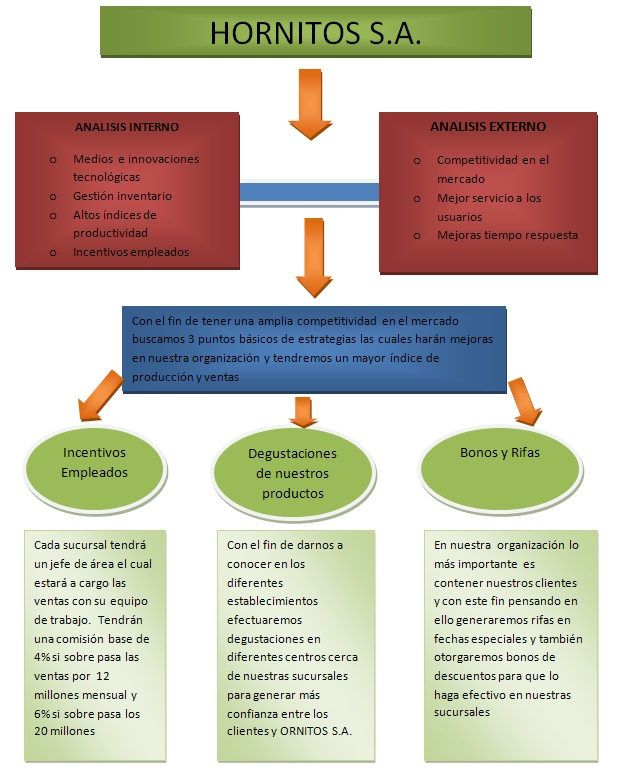
\includegraphics[width=0.60\textwidth]{images/Dibujo.jpg}
%el caption es para el texto que aparece debajo de la imagen
	\caption{Plan estrategico}
%label es para darle una referencia, por ejemplo si uno dice "como se puede ver en la imagen a1"
	\label{fig:Plan estrategico}
\end{figure}%
Hornitos S.A. Ha desarrollado una campa\~na la cual se dividir\'a en 3 partes las cuales buscara tener  por medio de los clientes una preferencia en nuestros productos e incentivar a nuestros trabajadores a tener mayor entrega con la organizaci\'on estar\'iamos hablando de tres proyectos los cuales buscaran un mejor \'ambito para la organizaci\'on.%
\\%
	
	\begin{itemize}
		\item Incentivos empleados.
		\item Degustaciones.
		\item bonos y rifas.
	\end{itemize}
	
\subsection{Incentivos empleados:}Cada sucursal tendr\'a un jefe de \'area el cual estar\'a a cargo las ventas con su  respectivo equipo de trabajo.  Tendr\'an una comisi\'on base de ventas pero con un incentivo adicional para los trabajadores y el jefe de la sucursal si logra sobre pasar ventas mensuales a 12 millones.%
\subsection{Degustaciones:} Con el fin de promocionar nuestro producto y generar una mayor demanda de ventas  efectuaremos degustaciones en diferentes centros cerca de nuestras sucursales para generar m\'as confianza entre los clientes y as\'i ser preferidos para ellos.
%
\subsection{Bonos y Rifas:} En nuestra  organizaci\'on lo m\'as importante es contener nuestros clientes y con este fin pensando en ello generaremos rifas en fechas especiales y tambi\'en otorgaremos bonos de descuentos para que lo haga efectivo en nuestras sucursales solo para la fidelidad de nuestros clientes 
\\%
\\%

%
\newpage%
\section{Reportes}
\begin{figure}[htbp]
%centering es para centrar la imagen
	\centering
%aca es donde se incluye la imagen, se da el ancho(width), \textwidth significa que con repescto al tamano del
%texto y luego la ruta, relativa siempre es decir, a partir de donde se esta, como images esta ahi
%dentro, solo se usa desde images y ojala nada de espacios en el nombre de la imagen
		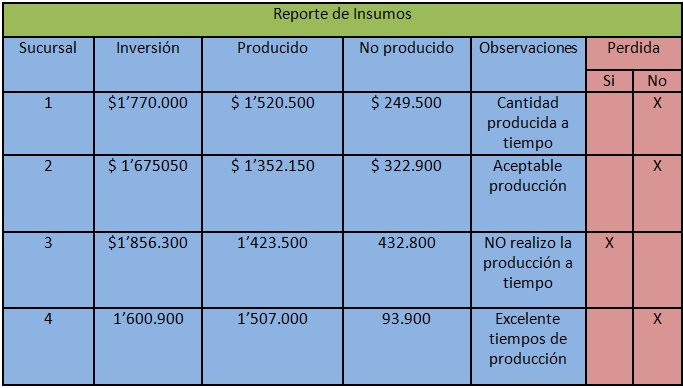
\includegraphics[width=0.60\textwidth]{images/REPORTEDEINSUMO.jpg}
%el caption es para el texto que aparece debajo de la imagen
	\caption{Reporte de insumo}
%label es para darle una referencia, por ejemplo si uno dice "como se puede ver en la imagen a1"
	\label{fig:Reporte de insumo}
\end{figure}%
\\%
\\%
\\%
\\%
\begin{figure}[htbp]
%centering es para centrar la imagen
	\centering
%aca es donde se incluye la imagen, se da el ancho(width), \textwidth significa que con repescto al tamano del
%texto y luego la ruta, relativa siempre es decir, a partir de donde se esta, como images esta ahi
%dentro, solo se usa desde images y ojala nada de espacios en el nombre de la imagen
		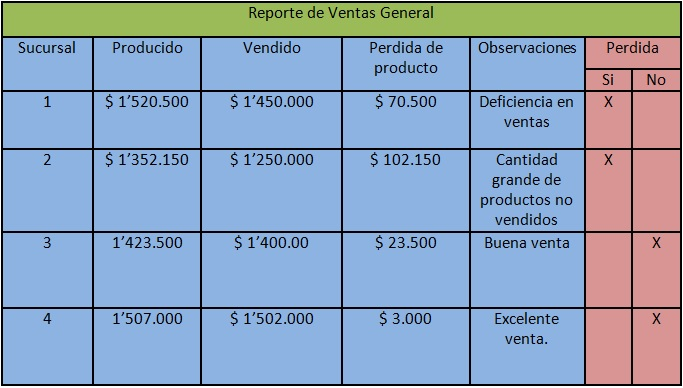
\includegraphics[width=0.60\textwidth]{images/REPORTEDEVENTASGENERAL.jpg}
%el caption es para el texto que aparece debajo de la imagen
	\caption{Reporte de ventas general}
%label es para darle una referencia, por ejemplo si uno dice "como se puede ver en la imagen a1"
	\label{fig:Reporte de ventas general}
\end{figure}%
\\%
\\%
\\%
\\%
\begin{figure}[htbp]
%centering es para centrar la imagen
	\centering
%aca es donde se incluye la imagen, se da el ancho(width), \textwidth significa que con repescto al tamano del
%texto y luego la ruta, relativa siempre es decir, a partir de donde se esta, como images esta ahi
%dentro, solo se usa desde images y ojala nada de espacios en el nombre de la imagen
		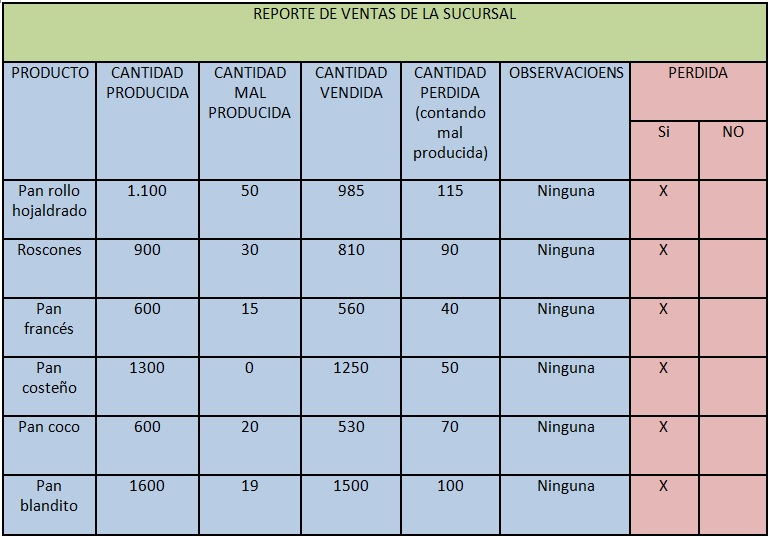
\includegraphics[width=0.60\textwidth]{images/REPORTEDEVENTASDELASUCURSAL.jpg}
%el caption es para el texto que aparece debajo de la imagen
	\caption{Reporte de ventas de una sucursal}
%label es para darle una referencia, por ejemplo si uno dice "como se puede ver en la imagen a1"
	\label{fig:Reporte de ventas de una sucursal}
\end{figure}%
\newpage%
\section{Diagrama de GANTT}
%
\mbox{}
\newpage%
%
\mbox{}
\newpage%
%
\section{Recursos}
%
\mbox{}
\newpage%
\mbox{}
\newpage%
\mbox{}
\newpage%
\mbox{}
\newpage%
\section{Presupuesto}
%
\mbox{}
\newpage%
%
\mbox{}
\newpage%
%
\section{Cronograma}
%
\mbox{}
\newpage%
\mbox{}
\newpage%
\mbox{}
\newpage%
\mbox{}
\newpage%
\newpage
\pagestyle{fancy}
\chapter{An\'alisis del sistema}
\section{Identificaci\'on de problemas y oportunidades b\'asicas}
En el estudio del sistema, se encontraron los siguientes problemas:%
\\
\begin{itemize}
\item El sistema debe ser flexible y parametrizable.%
\item El volumen del flujo de datos es muy grande.%
\item El registro de las ventas puede llegar a no estar acorde a la realidad.%
\item Los participantes pueden llegar a perder la tarjeta en la que se les realiza la consignaci\'on.%
\end{itemize}%
%
\begin{figure}[htbp]
%centering es para centrar la imagen
	\centering
%aca es donde se incluye la imagen, se da el ancho(width), \textwidth significa que con repescto al tamano del
%texto y luego la ruta, relativa siempre es decir, a partir de donde se esta, como images esta ahi
%dentro, solo se usa desde images y ojala nada de espacios en el nombre de la imagen
		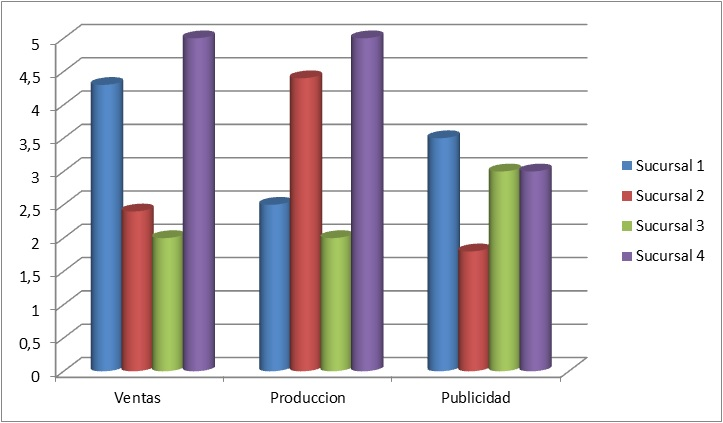
\includegraphics[width=0.60\textwidth]{images/Eficienciadelasucursal.jpg}
%el caption es para el texto que aparece debajo de la imagen
	\caption{Eficiencias de las sucursales}
%label es para darle una referencia, por ejemplo si uno dice "como se puede ver en la imagen a1"
	\label{fig:eficienciasucursales}
\end{figure}%
%
\section{Evaluaci\'on del beneficio del proyecto}
Lo beneficios de el sistema de informaci\'on que se va a implementar nos permitir\'a consultar, observar y verificar la informaci\'on de la compa\~n\'ia en tiempo real y efectiva, de tal forma que estos procesos puedan ser flexibles y f\'acil de manejar para el usuario, esto nos lleva a que se Incrementara  el entendimiento del uso de las Tecnolog\'ias de Informaci\'on en la organizaci\'on y posteriormente  incrementar las ventas; para llevar esto a cabo, es necesario ser el primero en proporcionar informaci\'on a clientes potenciales sobre un producto en particular. y mantener una relaci\'on con ellos a trav\'es de informaci\'on permanente.%
%
\subsection{?`Vale la pena trabajar en este proyecto?}
Hoy en d\'ia se esta tomando conciencia de la importancia dentro de las organizaciones de manejar los ambientes de negocio implementando un sistema de informaci\'on, lo fundamental para una compa\~n\'ia es un mercado globalizado a nivel competitivo, que tanto la estrategia de negocios y estrategias tecnol\'ogicas est\'en bajo un mismo esquema.%
\\%
\\%
Por lo anterior vale la pena trabajar en este proyecto ya que se ve reflejado la fusi\'on de estas dos estrategias, por una parte se esta trabajando los procesos del negocio y por el otro, se menejara un sistema que ayudar\'a a que todos estos procesos se realicen en forma automatizada, con el fin de alcanzar las metas y objetivos de la empresa.%
%
\subsection{?`Solucionar\'a los problemas?}
Uno de los principales inconvenientes de la organizaci\'on es que tiene varias sucursales las cuales no tienen un sistema que las haga cordinar unas a otras para mayor efectividad esto se produjo por la expancion de la organizacion de forma rapida, pero al llegar a un tama\~no tan grande empezo a crear se algunas deficiencias la cuales se pueden solucionar con un sistema de informacion para que este se encargue de dicha administracion de esta organizacion y generar mejor competitividad frente a otras organizaciones grandes. ya que este sistema generar mayor control de las ventas de forma mas organizada y consisa. y por medio de reportes llegar a tomar decisiones que ayuden a la organizacion a ser mas estable.%
%
\subsection{Agregar valor al proceso}
Se agrega valor en los siguientes aspectos:%
\begin{enumerate}
	\item Proporcionando informacion adicional para la alta gerencia la cual ayuda para la toma de decisiones.
	\item Identificando inconvenientes que si resuelven y mejora la competencia y el incremento de las venta.
	\item Identificando las oportunidades de mejora en el \'area de ventas.
\end{enumerate}%
%
\section{Dominio del problema}
El sistema que es implementado de forma sencilla no tan complejo ya que son pocos procesos que intervienen; siendo asi un sistema con escasamente 2 actores, los clientes y el ususario del sistema que puede ser gerente de mercadeo, administrador del sistema o gerente de ventas.%
%
%\begin{figure}[htbp]
%	\centering
%		\includegraphics[width=0.60\textwidth]{images/contexto.png}
%	\caption{Diagrama de contexto del dominio del problema}
%	\label{fig:contexto}
%\end{figure}%
%
%
%\begin{figure}[htbp]
%	\centering
%		\includegraphics[width=0.60\textwidth]{images/problemasoportunidades.png}
%	\caption{Matriz de problemas y oportunidades b\'asicas}
%	\label{fig:anaproblemas}
%\end{figure}%
%
\section{An\'alisis de el proceso del negocio}
	\begin{itemize}
		\item Inventarios
		\item Produccion
		\item Nomina
		\item Ventas
	\end{itemize}
\subsection{Inventarios:} En este proceso se gestionara dos tipos de inventarios:
	\begin{itemize}
		\item \textbf{Inventario de insumo:} en este inventario se manejan todos los productos necesarios para la producci\'on teniendo en cuenta cuando se va a gastar  para hacer dicha producci\'on y as\'i tener el control necesario de estos. En este proceso es fundamental implementar este sistema ya que es la parte inicial de la producci\'on y as\'i evitar riegos dentro de los procesos de producci\'on.
		\\%
		\\%
			Otro prop\'osito fundamental al generar este sistema dentro de los procesos que se encuentran en el inventario de insumos es automatizarlo para que facilite su utilizaci\'on, creaci\'on de reportes para saber si esta siendo efectiva la producci\'on y rentable dependiendo de la sucursal ya que en cada sucursal va tener una tasa de producci\'on diferente, Lo cual es fundamental para la toma de decisiones ya que si en una sucursal tiene una taza de producci\'on mas grande de la que se esta ingresando ya que puede afectar en este. 
		\\%
		\\%
		Al automatizar este proceso podemos saber que producto requiere de m\'as insumo que otro, y as\'i poder generar reportes y controles. 
		\\%
		\\%
		\textbf{Ejemplo grafico inventario de insumos por d\'ia de varias sucursales de la misma organizaci\'on.}
		\item \textbf{Inventario de producci\'on:} en  este inventario se manejan los productos ya producidos debidamente controlados por el sistema, como por ejemplo la cantidad de panes producidos de un tipo. La automatizaci\'on de este proceso ayuda a saber la cantidad que se esta produciendo, cantidad que se esta vendiendo, y cantidad que se esta perdiendo.
		\\%
		\\%
				\textbf{El siguiente grafico muestra en una sucursal la cantidad producida de un producto, cantidad vendida, y cantidad no vendida.}
	\end{itemize}
	\subsection{Producci\'on:}En este proceso se ejecuta al tener todos los inventarios insumos, y así empezar a producci\'on y toda la informaci\'on referente a la producci\'on es guardada en el inventario de producci\'on, en este proceso solo se encargara de convertir la materia prima en el producto.	
\\%
\\%
Al implementarse este sistema en este proceso tendr\'a varios controles, tales como: higiene de producto, mantenimiento de maquinaria. Al realizar todo este proceso podemos realizar los reportes por medio de graficas, estos reportes realizados son de todas las sucursales y esto nos mostrara que sucursal es mas eficiente, cual puede estar en mucha perdida para si tomar decisiones con respecto a estos reportes como por ejemplo si una sucursal gr\'aficamente esta descendiendo se puede llegar a tomar una decisi\'on de cerrar la sucursal por perdida.
\subsection{Nomina:}en este proceso gestionara la nomina de los empleados, y as\'i tener un control apropiado a todos los empleados, como por ejemplo saber si un empleado esta cumpliendo con sus horas que se le asignan por mes y pagos realizados a los clientes, de este proceso tambi\'en se generan reportes para saber que tasa de inversi\'on se esta haciendo en los empleados.
\subsection{Ventas:}en este proceso se gestionara toda las ventas, cantidad vendida, pedidos dependiendo de la sucursal, cantidad de clientes por d\'ia, d\'ias mas rentables y toda esta estad\'istica se obtiene de este proceso que sirve para poder realizar cambios de atenci\'on o mejorar productos, dependiendo si esta llegando la cantidad suficiente de clientes, tambi\'en podemos saber que cliente es mas frecuente y asi poder dar beneficios adionales para mantener el cliente por mas tiempo. Tambi\'en se puede puede saber que sucursal tiene mas taza de clientes.
\\%
\\%
Adicional a todos estos procesos tambi\'en se tiene un proceso el cual maneja todos los gasto fijos que va teniendo la organizaci\'on tales como impuestos, servicios, todo estos se manejara tambi\'en en un \'unico reporte el cual contiene todo los gastos e inversiones y  ventas y ganancias dentro de toda la organizaci\'on.
\\%
\\%
	\textbf{Ejemplo grafico de que tan eficiente es cada sucursal.}
%
\newpage%
\subsection{Diagramas de flujo}
%\begin{figure}[htbp]
%	\centering
%		\includegraphics[width=0.60\textwidth]{images/cuadritoese.png}
%	\caption{Proceso actual}
%	\label{fig:cuadritoese}
%\end{figure}%
%
\newpage%
\section{Identificaci\'on de requerimientos}
\subsection{Requerimientos no funcionales}
%\begin{figure}[htbp]
%	\centering
%		\includegraphics[width=1.00\textwidth]{images/nofuncionales.png}
%	\caption{Requerimientos no funcionales}
%	\label{fig:reqnofuncionales}
%\end{figure}%
%
\newpage%
\subsection{Requerimientos funcionales}
%\begin{figure}[htbp]
%	\centering
%		\includegraphics[width=1.00\textwidth]{images/funcionales.png}
%	\caption{Requerimientos funcionales}
%	\label{fig:reqfuncionales}
%\end{figure}%
%
\newpage%
\section{Priorizaci\'on de requerimientos del sistema}
%\begin{figure}[htbp]
%	\centering
%		\includegraphics[width=1.00\textwidth]{images/requerimientossitema.png}
%	\caption{Requerimientos del sistema}
%	\label{fig:reqsistema}
%\end{figure}%
%
\newpage
\pagestyle{fancy}
\chapter{ERP como soluci\'on adecuada}
%
La necesidad del negocio se puede resumir en los siguientes puntos:%
%
\begin{itemize}
\item Gesti\'on y soporte de los procesos para optimizaci\'on constante.
\item Control y seguimiento para permitir toma de desiciones.
\item Interconexi\'on e interoperabilidad entre las sucursales.
\end{itemize}
%
Teniendo en cuenta esto, la soluci\'on m\'as acertada es la implementaci\'on de un ERP, debido a las caracter\'isticas mencionadas anteriormente.%
\\%
\\%
Un sistema ERP permite gesti\'on unificada y descentralizada, permitiendo as\'i alcance a las sucursales sin traumatismos, permiti\'endoles ejercer como unidades independientes con un fin y una directriz en com\'un, con interacci\'on de forma asincr\'onica y en tiempo real, facilitando la gesti\'on y revisi\'on de los procesos.%

\newpage
\pagestyle{fancy}
\chapter{Reportes}
\begin{figure}[htbp]
%centering es para centrar la imagen
	\centering
%aca es donde se incluye la imagen, se da el ancho(width), \textwidth significa que con repescto al tamano del
%texto y luego la ruta, relativa siempre es decir, a partir de donde se esta, como images esta ahi
%dentro, solo se usa desde images y ojala nada de espacios en el nombre de la imagen
		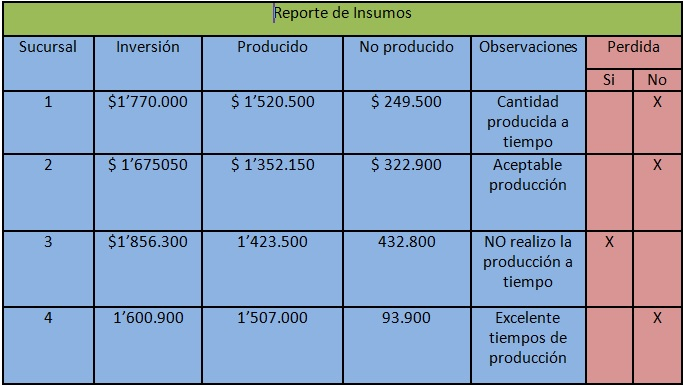
\includegraphics[width=0.60\textwidth]{images/REPORTEINSUMOS.jpg}
%el caption es para el texto que aparece debajo de la imagen
	\caption{Grafico de reporte de insumos}
%label es para darle una referencia, por ejemplo si uno dice "como se puede ver en la imagen a1"
	\label{fig:Grafico de reporte de insumos}
\end{figure}%
\begin{figure}[htbp]
%centering es para centrar la imagen
	\centering
%aca es donde se incluye la imagen, se da el ancho(width), \textwidth significa que con repescto al tamano del
%texto y luego la ruta, relativa siempre es decir, a partir de donde se esta, como images esta ahi
%dentro, solo se usa desde images y ojala nada de espacios en el nombre de la imagen
		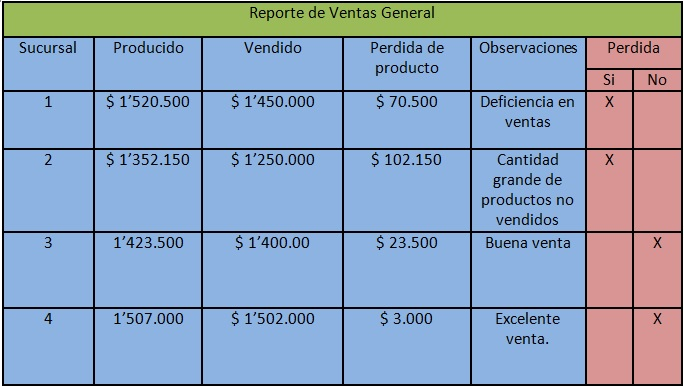
\includegraphics[width=0.60\textwidth]{images/REPORTEVENTASGENERAL.jpg}
%el caption es para el texto que aparece debajo de la imagen
	\caption{Reporte de ventas general}
%label es para darle una referencia, por ejemplo si uno dice "como se puede ver en la imagen a1"
	\label{fig:Reporte de ventas general}
\end{figure}%
\begin{figure}[htbp]
%centering es para centrar la imagen
	\centering
%aca es donde se incluye la imagen, se da el ancho(width), \textwidth significa que con repescto al tamano del
%texto y luego la ruta, relativa siempre es decir, a partir de donde se esta, como images esta ahi
%dentro, solo se usa desde images y ojala nada de espacios en el nombre de la imagen
		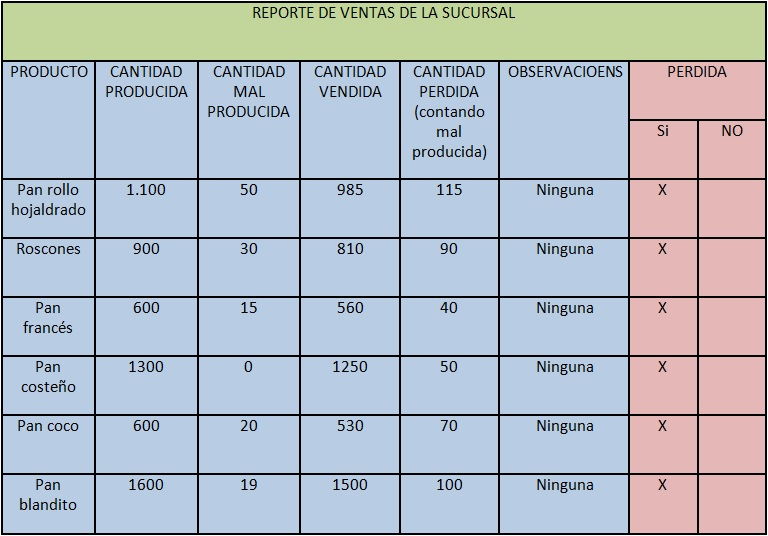
\includegraphics[width=0.60\textwidth]{images/REPORTEVENTASSUCURSAL.jpg}
%el caption es para el texto que aparece debajo de la imagen
	\caption{Reporte de ventas de una sucursal}
%label es para darle una referencia, por ejemplo si uno dice "como se puede ver en la imagen a1"
	\label{fig:Reporte de ventas de una sucursal}
\end{figure}%

%\newpage
%Otros apendices
%\bibliographystyle{abbrv}
%\bibliography{myblib}
%\clearemptydoublepage
\end{document}
